\documentclass[12pt]{beamer}
\newenvironment{ConCodigo}[1]
  {\begin{frame}[fragile,environment=ConCodigo]{#1}}
  {\end{frame}}
\graphicspath{{Imagenes/}{../Imagenes/}}
\usepackage[utf8]{inputenc}
\usepackage[spanish]{babel}
\usepackage{hyperref}
\usepackage{etex}
\reserveinserts{28}
\usepackage{amsmath}
\usepackage{amsthm}
\usepackage{mathtools}
\usepackage{multicol}
\usepackage{multirow}
\usepackage{tabulary}
\usepackage{booktabs}
\usepackage{nccmath}
\usepackage{biblatex}
\usepackage{epstopdf}
\usepackage{graphicx}
%\usepackage{enumitem,xcolor}
\usepackage{siunitx}
\sisetup{scientific-notation=true}
%\usepackage{fontspec}
\usepackage{lmodern}
\usepackage{float}
\usepackage[format=hang, font=footnotesize, labelformat=parens]{caption}
\usepackage[autostyle,spanish=mexican]{csquotes}
\usepackage{standalone}
\usepackage{blkarray}
\usepackage{algorithm}
\usepackage{algorithmic}
\usepackage{tikz}
\usepackage[siunitx]{circuitikz}
\usetikzlibrary{arrows,patterns,shapes}
\usetikzlibrary{decorations.markings}
\usetikzlibrary{arrows}
\usepackage{color}
\usepackage{xcolor}
%\usepackage{beton}
%\usepackage{euler}
%\usepackage[T1]{fontenc}
\usepackage[sfdefault]{roboto}  %% Option 'sfdefault' only if the base font of the document is to be sans serif
\usepackage[T1]{fontenc}
\renewcommand*\familydefault{\sfdefault}
\DeclareGraphicsExtensions{.pdf,.png,.jpg}
\usepackage{hyperref}
\renewcommand {\arraystretch}{1.5}
\newcommand{\python}{\texttt{python}}
\usefonttheme[onlymath]{serif}
\setbeamertemplate{navigation symbols}{}
\usetikzlibrary{patterns}
\usetikzlibrary{decorations.markings}
\tikzstyle{every picture}+=[remember picture,baseline]
%\tikzstyle{every node}+=[inner sep=0pt,anchor=base,
%minimum width=2.2cm,align=center,text depth=.15ex,outer sep=1.5pt]
%\tikzstyle{every path}+=[thick, rounded corners]
\setbeamertemplate{caption}[numbered]
\newcommand{\ptm}{\fontfamily{ptm}\selectfont}
%Se usa la plantilla Warsaw modificada con spruce
\mode<presentation>
{
  \usetheme{Warsaw}
  \setbeamertemplate{headline}{}
  \useoutertheme{default}
  \usecolortheme{seahorse}
  \setbeamercovered{invisible}
}
% \AtBeginSection[]
% {
% \begin{frame}<beamer>{Contenido}
% \normalfont\mdseries
% \tableofcontents[currentsection]
% \end{frame}
%}

\usepackage{listings}
\lstset{ %
language=Python,                % choose the language of the code
basicstyle=\small,       % the size of the fonts that are used for the code
numbers=left,                   % where to put the line-numbers
numberstyle=\footnotesize,      % the size of the fonts that are used for the line-numbers
stepnumber=1,                   % the step between two line-numbers. If it is 1 each line will be numbered
numbersep=5pt,                  % how far the line-numbers are from the code
backgroundcolor=\color{white},  % choose the background color. You must add \usepackage{color}
showspaces=false,               % show spaces adding particular underscores
showstringspaces=false,         % underline spaces within strings
showtabs=false,                 % show tabs within strings adding particular underscores
frame=single,   		% adds a frame around the code
tabsize=4,  		% sets default tabsize to 2 spaces
captionpos=b,   		% sets the caption-position to bottom
breaklines=true,    	% sets automatic line breaking
breakatwhitespace=false,    % sets if automatic breaks should only happen at whitespace
escapeinside={\#}{)}          % if you want to add a comment within your code
}

\title{Tema 1 - Problemas de la f\'{i}sica}
\subtitle{Curso de F\'{i}sica Computacional}
\author[]{M. en C. Gustavo Contreras May\'{e}n}
%\email{curso.fisica.comp@gmail.com}
%\ptsize{10}
\begin{document}
\maketitle
\fontsize{14}{14}\selectfont
\spanishdecimal{.}
\AtBeginSection[]
{
\begin{frame}{Contenido}
\tableofcontents[ 
    currentsubsection, 
    hideothersubsections, 
    sectionstyle=show/hide, 
    subsectionstyle=show/shaded, 
    hideothersubsections
    ] 
\end{frame}
}
\section{Abordar problemas de la f\'{i}sica}
\begin{frame}
\frametitle{Abordar problemas de la f\'{i}sica}
De manera paralela a los conceptos importantes del curso, es necesario iniciar el trabajo de plantear algoritmos de soluci\'{o}n a problemas de la f\'{i}sica.
\\
\medskip
La mejor manera de aprender, es sentarse a programar. Debe de tenerse la calma para ello, la idea es ir perfeccionando las propuestas de soluci\'{o}n, es importante señalar que la inspiraci\'{o}n divina, no se da siempre.
\end{frame}
\begin{frame}[fragile]
\frametitle{Proceso de programaci\'{o}n}
El proceso de programaci\'{o}n consta de las actividades necesarias para escribir programas que funcionen adecuadamente como soluci\'{o}n a un problema particular. \footnote{Amparo L\'{o}pez Gaona, \textit{Introducci\'{o}n al desarrollo de programas con Java}, 3a. Ed., La Prensa de Ciencias, México D.F. 2013.}
\begin{enumerate}[<+->]
\item Definici\'{o}n del problema.
\item Diseño de la soluci\'{o}n.
\item Codificaci\'{o}n.
\item Depuraci\'{o}n.
\item Mantenimiento.
\end{enumerate}
\end{frame}
\begin{frame}
\frametitle{Definici\'{o}n del problema}
Aqu\'{i} se especifica qu\'{e} es lo que debe de hacer el programa.
\\
\bigskip
Este primer paso puede parecer trivial aunque no lo es. La comprensi\'{o}n exacta de lo que se necesita hacer es requisito indispensable para crear una soluci\'{o}n funcional.
\\
\medskip
En ocasiones, se ignora esta fase y se comienza a escribir un programa sin tener en claro el problema a resolver.
\end{frame}
\begin{frame}
\frametitle{Diseño de la soluci\'{o}n}
En esta fase se indica una forma de satisfacer, mediante un programa, los requerimientos establecidos en la etapa anterior.
\\
\bigskip
El diseño de un programa es un proceso al que muchas veces no se le da la importancia y de ah\'{i} que en las etapas posteriores se tengan muchos problemas.
\\
\medskip
En el diseño es necesario identificar los principales componentes de la soluci\'{o}n y la relaci\'{o}n entre ellos.
\end{frame}
\begin{frame}
\frametitle{Codificaci\'{o}n}
Una vez que se tiene el diseño de la soluci\'{o}n, se procede a traducirlo a un lenguaje de programaci\'{o}n.
\\
\bigskip
Esta tarea se conoce como codificaci\'{o}n o implementaci\'{o}n. En muchas ocasiones, uno se centra \'{u}nicamente en esta etapa aunque, como se puede ver, el proceso de programar es mucho m\'{a}s complejo y creativo.
\end{frame}
\begin{frame}[fragile]
Es recomendable acostumbrarse desde el inicio a escribir programas que sean f\'{a}cilmente entendibles por otras personas; podemos apoyarnos con lo siguiente:
\begin{enumerate}[<+->]
\item Los programas deben de tener una estructura clara.
\item El c\'{o}digo debe estar organizado y presentado de manera que sea f\'{a}cil su lectura.
\item El c\'{o}digo debe de estar documentado.
\end{enumerate}
\end{frame}
\begin{frame}
\frametitle{Depuraci\'{o}n}
El siguiente paso en el desarrollo de un programa es la depuraci\'{o}n que consiste en verificar que el algoritmo y el programa sean adecuados. No importa que tan bonito est\'{e} el programa, si no produce los resultados deseados, simplemente no sirve.
\\
\bigskip
Depurar implica descubrir, localizar y corregir todos los errores que causen que un programa produzca resultados incorrectos o que no produzca ning\'{u}n resultado.
\end{frame}
\begin{frame}
\frametitle{Mantenimiento}
En los programas y trabajos escolares, la tarea termina en el paso anterior, pero en la vida real no es as\'{i}. La etapa de mantenimiento consiste en supervisar la operaci\'{o}n de un programa, corregir cualquier error encontrado durante su uso continuo o efectuar modificaciones al mismo, con el prop\'{o}sito de que realice m\'{a}s tareas o de manera diferente a las que ten\'{i}an contempladas originalmente.
\end{frame}
\section{Un problema de Mec\'{a}nica}
\begin{frame}
\frametitle{Un problema de Mec\'{a}nica}
Supongamos que tenemos una part\'{i}cula de masa $m$ que est\'{a} confinada a moverse a lo largo del eje $x$, bajo una fuerza $f(x)$. Sabemos de la ley de Newton que
\begin{equation}\label{Eqfuerza}
f = ma = m \dfrac{dv}{dt}
\end{equation}
donde $a$ es la aceleraci\'{o}n y $v$ la velocidad de la part\'{i}cula respectivamente, $t$ es el tiempo.
\\
\medskip
Si dividimos el tiempo en pequeños intervalos iguales $\tau = t_{i+1} - t_{i}$, sabemos que la velocidad en el tiempo $t_{i}$, est\'{a} dada de manera aproximada por el promedio de la velocidad en el intervalo de tiempo $[t_{i}, t_{i+1}]$
\end{frame}
\begin{frame}
Por lo que
\begin{equation}\label{Eqvelocidad}
v_{i} \simeq \dfrac{x_{i+1}-x_{i}}{t_{i+1}-t_{i}} = \dfrac{x_{i+1}-x_{i}}{\tau}
\end{equation}
La aceleraci\'{o}n de la part\'{i}cula es aproximadamente el promedio de la aceleraci\'{o}n en el mismo intervalo
\begin{equation}\label{Eqaceleracion}
a_{i} \simeq \dfrac{v_{i+1}-v_{i}}{t_{i+1}-t_{i}} = \dfrac{v_{i+1}-v_{i}}{\tau}
\end{equation}
donde $\tau$ es muy pequeño.
\end{frame}
\begin{frame}
El algoritmo m\'{a}s sencillo para determinar la posici\'{o}n y velocidad de la part\'{i}cula en el tiempo $t_{1i+1}$, a partir de las cantidades correspondientes al tiempo $t_{i}$, se obtiene luego de combinar las ecuaciones (\ref{Eqfuerza}), (\ref{Eqvelocidad}) y (\ref{Eqaceleracion}), por lo que
\begin{eqnarray}
x_{i+1} &=& x_{i} + \tau v_{i} \label{Eqposicion} \\
v_{i+1} &=& v_{i} + \dfrac{\tau}{m} f_{i} \label{Eqvelocidadr}
\end{eqnarray}
donde $f_{i} = f(x_{i})$
\end{frame}
\begin{frame}
Si se proporciona la posici\'{o}n inicial y la velocidad de la part\'{i}cula y se buscan las cantidades correspondientes en alg\'{u}n momento posterior (problema de valor inicial), podemos obtenerlas de forma recursiva a partir del algoritmo dado en las ecuaciones (\ref{Eqposicion}) y (\ref{Eqvelocidadr}).
\end{frame}
\section{Ejercicio 1: Oscilador mec\'{a}nico}
\begin{frame}
\frametitle{Ejercicio 1: Oscilador mec\'{a}nico}
Por simplicidad, consideremos que la fuerza es $f(x) = -kx$, donde $k$ es la constante del resorte. Usemos $m=k=1$. Queremos describir la posici\'{o}n y velocidad de la part\'{i}cula en un intervalo de tiempo de 100 segundos. Las condiciones iniciales son las siguientes: $x(t=0) = 0$ y $v(t=0) = 1$.
\end{frame}
\begin{frame}[<+->]
\frametitle{Resolviendo el problema con Python}
¿Qu\'{e} es lo que tenemos?
\begin{itemize}
\item El intervalo de tiempo de $[0,100]$ segundos.
\item La posici\'{o}n y velocidad inicial.
\item Las expresiones para calcular los $x_{i+1}$ y $v_{i+1}$
\end{itemize}
\visible<4->{¿Qu\'{e} nos falta?}
\end{frame}
\begin{frame}[fragile]
\frametitle{Lo que nos falta}
\begin{itemize}[<+->]
\item Calcular para cada segundo en $[0,100]$ la posici\'{o}n y velocidad.
\item Guardar esos valores en un alg\'{u}n lado.
\item Graficar los resultados.
\end{itemize}
\end{frame}
\begin{frame}[fragile]
\frametitle{Uso de los m\'{o}dulos para nuestro programa}
\begin{lstlisting}
import matplotlib.pyplot as plt
from math import pi
\end{lstlisting}
\end{frame}
\begin{frame}[fragile]
\frametitle{Usando la informaci\'{o}n que nos proporciona el problema}
\begin{lstlisting}
n = 100

x = []
v = []

dt = 2* pi/n

x.append(0)
v.append(1)
\end{lstlisting}
\end{frame}
\begin{frame}[fragile]
\frametitle{Ciclo de iteraci\'{o}n para los nuevos valores}
\begin{lstlisting}
for i in range(n-1):
    xi = x[i] + v[i]*dt
    vi = v[i] - x[i]*dt
    
    x.append(xi)
    v.append(vi)
\end{lstlisting}
\end{frame}
\begin{frame}[fragile]
\frametitle{Generaci\'{o}n de una gr\'{a}fica}
\begin{lstlisting}
plt.plot(x, "ro-", label="Posicion")
plt.plot(v, "b+-", label="Velocidad")
plt.legend(loc="upper right")
plt.xlabel("tiempo")
plt.show()
\end{lstlisting}
\end{frame}
\begin{frame}
\frametitle{Resultado del problema}
\begin{figure}
	\centering
	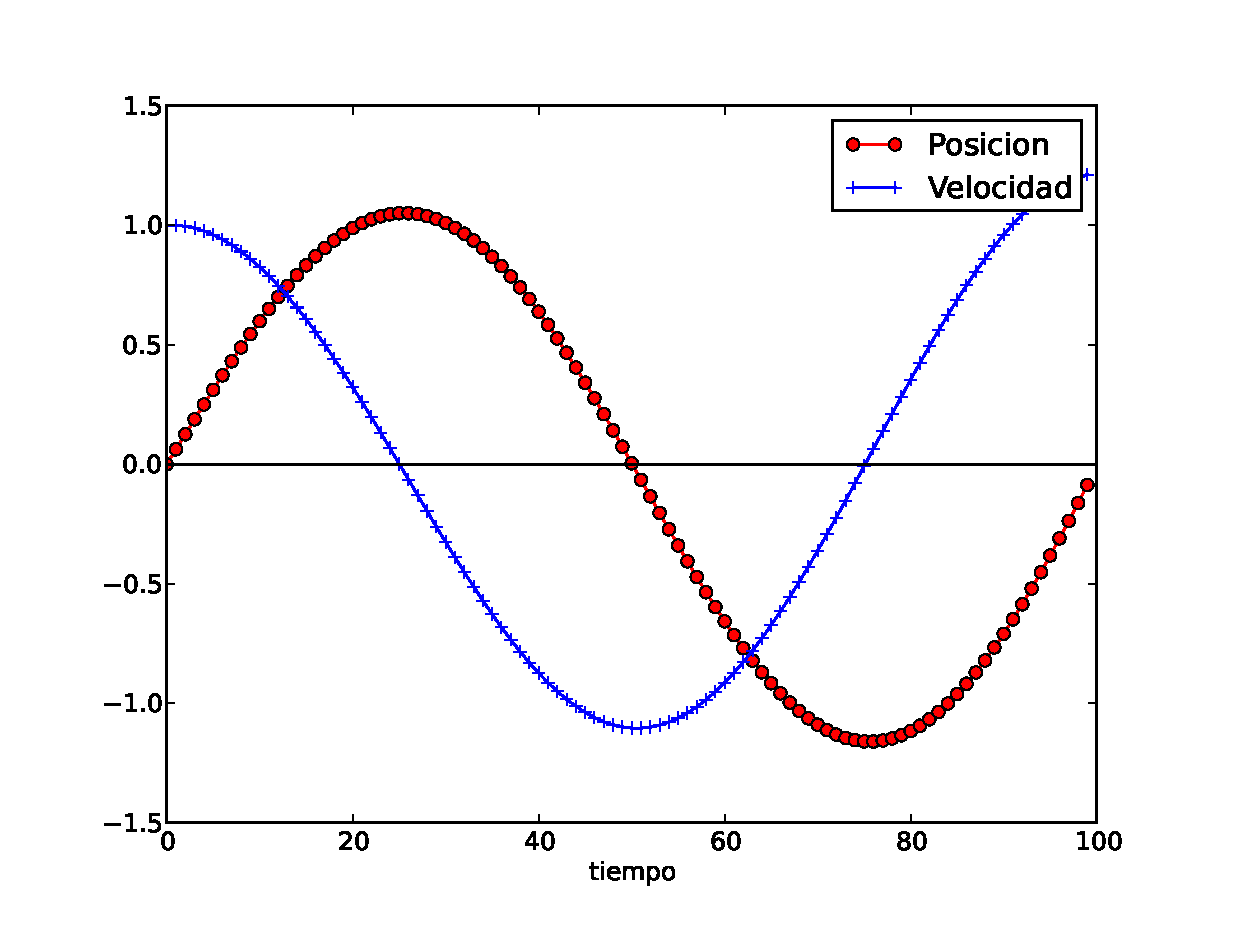
\includegraphics[scale=0.5]{Imagenes/EjerMecanica01.eps} 
\end{figure}
\end{frame}
\section{Ejecicio 2: Efecto de la resistencia del aire}
\begin{frame}
\frametitle{Ejecicio 2: Efecto de la resistencia del aire}
La bicicleta es una forma muy eficiente de transporte, este es un hecho bien conocido por cualquier persona que monta una. Nuestro objetivo en este ejercicio es comprender los factores que determinan la velocidad m\'{a}xima de una bicicleta y estimar la velocidad de un caso real.
\\
\bigskip
Comenzaremos haciendo caso omiso de la fricci\'{o}n; tendremos que añadirlo al final, por supuesto, pero debemos primero entender c\'{o}mo lidiar con el caso m\'{a}s simple y sin fricci\'{o}n.
\end{frame}
\begin{frame}
La ecuaci\'{o}n de movimiento corresponde a la segunda ley de Newton, que escribimos de la forma
\begin{equation}\label{EqNewton2}
\dfrac{dv}{dt} = \dfrac{F}{m}
\end{equation}
donde $v$ es la velocidad, $m$ es la masa de la combinaci\'{o}n de la bicicleta-conductor, $t$ es el tiempo, y $F$ es la fuerza en la bicicleta que viene del esfuerzo del conductor (en este caso vamos a suponer que la bicicleta se mueve sobre un terreno plano)
\end{frame}
\begin{frame}
Tratar correctamente a $F$ se complica por la mec\'{a}nica de la bicicleta, ya que la fuerza ejercida por el ciclista se transmite a las ruedas por medio del plato, engranajes, cadena, etc. Esto hace que sea muy dif\'{i}cil derivar una expresi\'{o}n exacta para $F$.
\\
\medskip
Sin embargo, hay otra manera de abordar este problema que evita la necesidad de conocer la fuerza. Este enfoque alternativo implica la formulaci\'{o}n del problema en t\'{e}rminos de la potencia generada por el ciclista.
\\
\medskip
Estudios fisiol\'{o}gicos de ciclistas de carreras han demostrado que estos atletas son capaces de producir una potencia de salida de aproximadamente 400 watts durante largos per\'{i}odos de tiempo ($\sim 1$ h)
\end{frame}
\begin{frame}
Usando las ideas de trabajo-energ\'{i}a podemos reescribir (\ref{EqNewton2}) como
\begin{equation}\label{EqPotencia}
\dfrac{dE}{dt} = P
\end{equation}
donde $E$ es la energ\'{i}a total, $P$ es la potencia de salida del ciclista. Para un trayecto plano la energ\'{i}a es totalmente cin\'{e}tica, es decir, $E = \frac{1}{2} m v^{2}$, y $\frac{dE}{dt} = mv (\frac{dv}{dt})$, usando esto en (\ref{EqPotencia}), resulta
\begin{equation}\label{EqPotenciavel}
\dfrac{dv}{dt} = \dfrac{P}{mv}
\end{equation}
\end{frame}
\begin{frame}
Si $P$ es una constante, la ecuaci\'{o}n (\ref{EqPotenciavel}), se puede resolver de manera anal\'{i}tica, rearreglando t\'{e}rminos:
\begin{equation}\label{EqIntegral}
\int_{v_{0}}^{v} v' dv' = \int_{0}^{t} \dfrac{P}{m} dt'
\end{equation}
donde $v_{0}$ es la velocidad de la bicicleta en $t=0$. Integrando ambos lados de la ecuaci\'{o}n y resolviendo para $v$, tenemos
\begin{equation}\label{Eqvres}
v = \sqrt{v_{0}^{2} + 2 P \dfrac{t}{m}}
\end{equation}
\end{frame}
\begin{frame}
Si bien esta es la soluci\'{o}n correcta de la ecuación de movimiento (\ref{EqPotenciavel}), nuestro trabajo no puede concluir aqu\'{i}, ya que predice que la velocidad se incrementar\'{a} sin l\'{i}mite para tiempos muy largos.
\\
\medskip
Vamos a corregir este resultado, cuando se generaliza el modelo se debe de incluir el efecto de la resistencia del aire. El nuevo t\'{e}rmino que vamos a añadir a la ecuaci\'{o}n de movimiento nos obliga a desarrollar una solución num\'{e}rica, as\'{i} que con eso en mente se considera un tratamiento numérico de (\ref{EqPotenciavel})
\end{frame}
\begin{frame}
Comenzamos con la forma de diferencias finitas para la derivada de la velocidad
\begin{equation}\label{Eqderivada}
\dfrac{dv}{dt} \simeq \dfrac{v_{i+1}-v_{i}}{\Delta t}
\end{equation}
donde asumimos que $\Delta t$ es paso discreto pequeño, y $v_{i}$ es la velocidad al tiempo $t_{i} \equiv i \Delta t$, por lo que de la ecuaci\'{o}n (\ref{EqPotenciavel})
\begin{equation}\label{Eqveli+1}
v_{i+1} = v_{i} + \dfrac{P}{m v_{i}} \Delta t
\end{equation}
\end{frame}
\begin{frame}
Dada la velocidad en un tiempo $i$ (es decir, $v_{i}$), podemos usar (\ref{Eqveli+1}) para calcular un valor \textit{aproximado} de la velocidad en el siguiente paso $v_{i+1}$.
\\
\medskip
Si conocemos la velocidad inicial $v_{0}$, podemos obtener $v_{1}$, $v_{2}$, y as\'{i} sucecivamente.
\end{frame}
\begin{frame}
\frametitle{Resultado de la velocidad sin fricci\'{o}n}
\begin{figure}
	\centering
	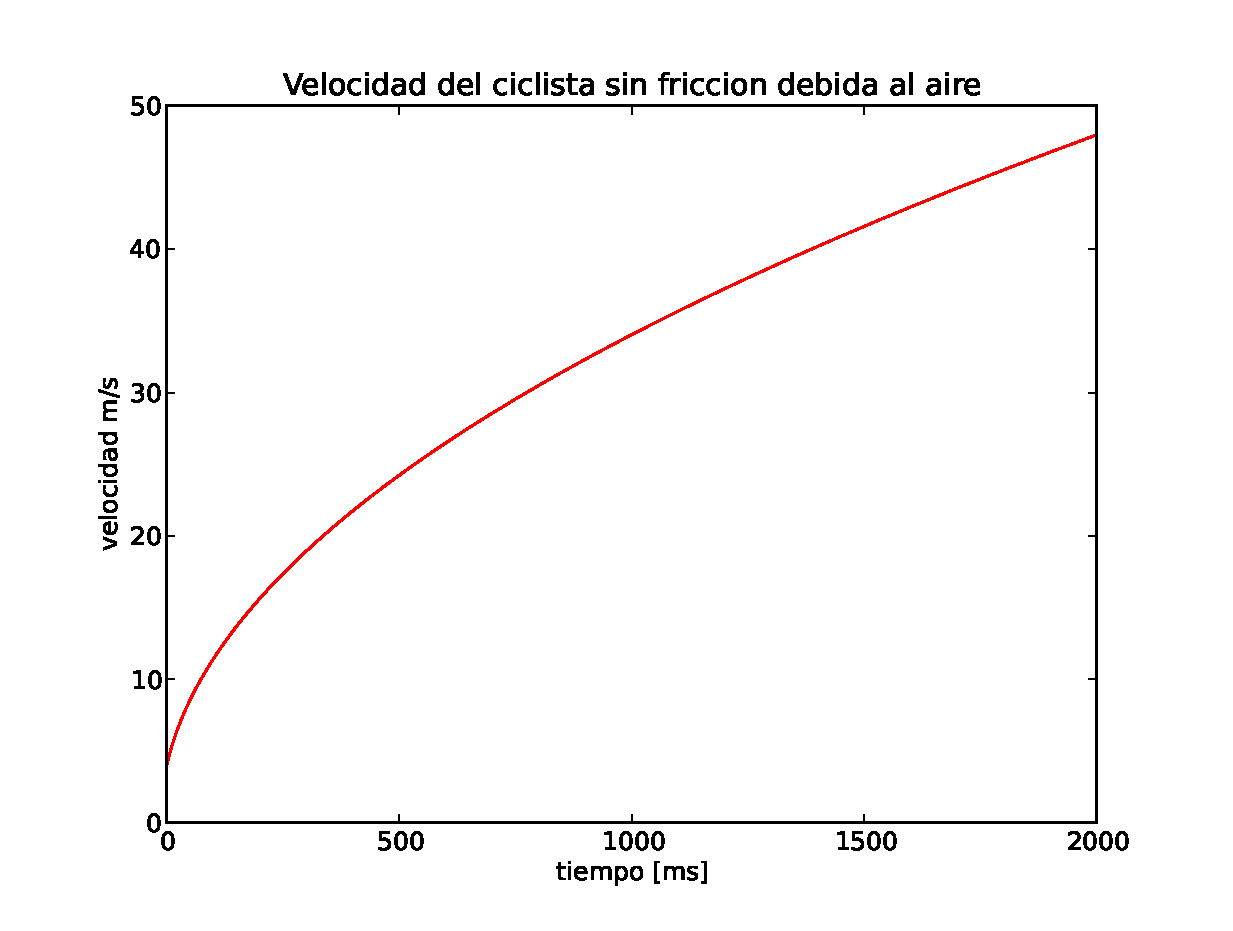
\includegraphics[scale=0.5]{EjerBicicleta01.eps}
\end{figure}
\end{frame}
\begin{frame}
\frametitle{Considerando la fricci\'{o}n del aire}
La fuerza debida a la fricci\'{o}n puede aproximarse de manera inicial como
\begin{equation}\label{EqFfriccion}
F_{a} \simeq - B_{1} v - B_{2} v^{2}
\end{equation}
Para velocidades muy bajas, el primer t\'{e}rmino es el que domina, y el coeficiente $B_{1}$ se puede calcular para objetos con formas sencillas.
\\
\medskip
Para una velocidad razonable $v^{2}$ el t\'{e}rmino domina sobre los dem\'{a}s, pero $B_{2}$ no puede calcularse exactamente en objetos sencillos como una pelota de beisbol, menos para una bicicleta.
\end{frame}
\begin{frame}
Podemos aproximar el valor de $B_{2}$ como sigue:
\\
\medskip
Si un objeto se mueve a trav\'{e}s de la atm\'{o}sfera y debe empujar fuera del camino el aire delante de \'{e}l. La masa de aire movido en el tiempo $dt$ es $m_{aire} \sim \rho Avdt$, donde $\rho$ es la densidad del aire y $A$ el \'{a}rea frontal del objeto. A este aire se le da una velocidad de orden $v$, y por lo tanto, su energ\'{i}a cin\'{e}tica es $E_{aire} \sim m_{aire} v^{2} /2$
\\
\medskip
Este es tambi\'{e}n el trabajo realizado por la fuerza de arrastre (la fuerza sobre el objeto debido a la resistencia del aire) en el tiempo $dt$, por lo $F_{a}vdt = E_{aire}$. Poniendo todo esto junto nos encontramos
\[ F_{a} \simeq - C \rho A v^{2} \]
\end{frame}
\begin{frame}
Incluyendo este t\'{e}rmino en la expresi\'{o}n para la velocidad
\begin{equation}\label{Eqvelifriccion}
v_{i+1} = v_{i} + \dfrac{P}{m v_{i}} \Delta t - \dfrac{C \rho A v_{i}^{2}}{m} \Delta t
\end{equation}
Ahora te toca implementar el c\'{o}digo, considerando $C = 0.5$ y $A=0.33$
\end{frame}
\begin{frame}
\frametitle{Comparando velocidades}
\begin{figure}
	\centering
	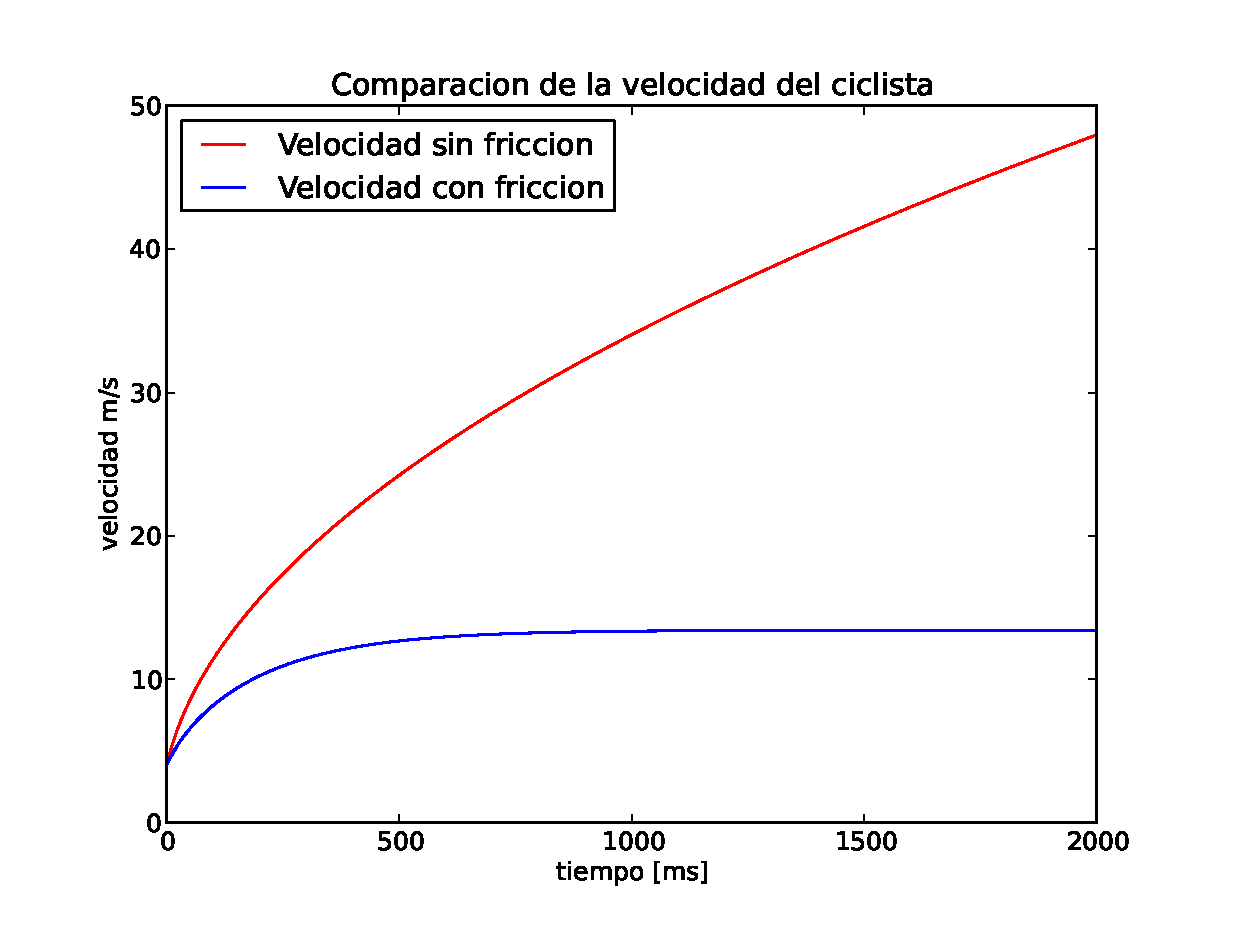
\includegraphics[scale=0.5]{EjerBicicleta02.eps}
\end{figure}
\end{frame}
\end{document}
